\documentclass{report}

\documentclass[12pt]{article}
\usepackage{array}
\usepackage{color}
\usepackage{amsthm}
\usepackage{eufrak}
\usepackage{lipsum}
\usepackage{pifont}
\usepackage{yfonts}
\usepackage{amsmath}
\usepackage{amssymb}
\usepackage{ccfonts}
\usepackage{comment} \usepackage{amsfonts}
\usepackage{fancyhdr}
\usepackage{graphicx}
\usepackage{listings}
\usepackage{mathrsfs}
\usepackage{setspace}
\usepackage{textcomp}
\usepackage{blindtext}
\usepackage{enumerate}
\usepackage{microtype}
\usepackage{xfakebold}
\usepackage{kantlipsum}
%\usepackage{draftwatermark}
\usepackage[spanish]{babel}
\usepackage[margin=1.5cm, top=2cm, bottom=2cm]{geometry}
\usepackage[framemethod=tikz]{mdframed}
\usepackage[colorlinks=true,citecolor=blue,linkcolor=red,urlcolor=magenta]{hyperref}

%//////////////////////////////////////////////////////
% Watermark configuration
%//////////////////////////////////////////////////////
%\SetWatermarkScale{4}
%\SetWatermarkColor{black}
%\SetWatermarkLightness{0.95}
%\SetWatermarkText{\texttt{Watermark}}

%//////////////////////////////////////////////////////
% Frame configuration
%//////////////////////////////////////////////////////
\newmdenv[tikzsetting={draw=gray,fill=white,fill opacity=0},backgroundcolor=none]{Frame}

%//////////////////////////////////////////////////////
% Font style configuration
%//////////////////////////////////////////////////////
\renewcommand{\familydefault}{\ttdefault}
\renewcommand{\rmdefault}{tt}

%//////////////////////////////////////////////////////
% Bold configuration
%//////////////////////////////////////////////////////
\newcommand{\fbseries}{\unskip\setBold\aftergroup\unsetBold\aftergroup\ignorespaces}
\makeatletter
\newcommand{\setBoldness}[1]{\def\fake@bold{#1}}
\makeatother

%//////////////////////////////////////////////////////
% Default font configuration
%//////////////////////////////////////////////////////
\DeclareFontFamily{\encodingdefault}{\ttdefault}{%
  \hyphenchar\font=\defaulthyphenchar
  \fontdimen2\font=0.33333em
  \fontdimen3\font=0.16667em
  \fontdimen4\font=0.11111em
  \fontdimen7\font=0.11111em}


%From M275 "Topology" at SJSU
\newcommand{\id}{\mathrm{id}}
\newcommand{\taking}[1]{\xrightarrow{#1}}
\newcommand{\inv}{^{-1}}

%From M170 "Introduction to Graph Theory" at SJSU
\DeclareMathOperator{\diam}{diam}
\DeclareMathOperator{\ord}{ord}
\newcommand{\defeq}{\overset{\mathrm{def}}{=}}

%From the USAMO .tex files
\newcommand{\ts}{\textsuperscript}
\newcommand{\dg}{^\circ}
\newcommand{\ii}{\item}

% % From Math 55 and Math 145 at Harvard
% \newenvironment{subproof}[1][Proof]{%
% \begin{proof}[#1] \renewcommand{\qedsymbol}{$\blacksquare$}}%
% {\end{proof}}

\newcommand{\liff}{\leftrightarrow}
\newcommand{\lthen}{\rightarrow}
\newcommand{\opname}{\operatorname}
\newcommand{\surjto}{\twoheadrightarrow}
\newcommand{\injto}{\hookrightarrow}
\newcommand{\On}{\mathrm{On}} % ordinals
\DeclareMathOperator{\img}{im} % Image
\DeclareMathOperator{\Img}{Im} % Image
\DeclareMathOperator{\coker}{coker} % Cokernel
\DeclareMathOperator{\Coker}{Coker} % Cokernel
\DeclareMathOperator{\Ker}{Ker} % Kernel
\DeclareMathOperator{\rank}{rank}
\DeclareMathOperator{\Spec}{Spec} % spectrum
\DeclareMathOperator{\Tr}{Tr} % trace
\DeclareMathOperator{\pr}{pr} % projection
\DeclareMathOperator{\ext}{ext} % extension
\DeclareMathOperator{\pred}{pred} % predecessor
\DeclareMathOperator{\dom}{dom} % domain
\DeclareMathOperator{\ran}{ran} % range
\DeclareMathOperator{\Hom}{Hom} % homomorphism
\DeclareMathOperator{\Mor}{Mor} % morphisms
\DeclareMathOperator{\End}{End} % endomorphism

\newcommand{\eps}{\epsilon}
\newcommand{\veps}{\varepsilon}
\newcommand{\ol}{\overline}
\newcommand{\ul}{\underline}
\newcommand{\wt}{\widetilde}
\newcommand{\wh}{\widehat}
\newcommand{\vocab}[1]{\textbf{\color{blue} #1}}
\providecommand{\half}{\frac{1}{2}}
\newcommand{\dang}{\measuredangle} %% Directed angle
\newcommand{\ray}[1]{\overrightarrow{#1}}
\newcommand{\seg}[1]{\overline{#1}}
\newcommand{\arc}[1]{\wideparen{#1}}
\DeclareMathOperator{\cis}{cis}
\DeclareMathOperator*{\lcm}{lcm}
\DeclareMathOperator*{\argmin}{arg min}
\DeclareMathOperator*{\argmax}{arg max}
\newcommand{\cycsum}{\sum_{\mathrm{cyc}}}
\newcommand{\symsum}{\sum_{\mathrm{sym}}}
\newcommand{\cycprod}{\prod_{\mathrm{cyc}}}
\newcommand{\symprod}{\prod_{\mathrm{sym}}}
\newcommand{\Qed}{\begin{flushright}\qed\end{flushright}}
\newcommand{\parinn}{\setlength{\parindent}{1cm}}
\newcommand{\parinf}{\setlength{\parindent}{0cm}}
% \newcommand{\norm}{\|\cdot\|}
\newcommand{\inorm}{\norm_{\infty}}
\newcommand{\opensets}{\{V_{\alpha}\}_{\alpha\in I}}
\newcommand{\oset}{V_{\alpha}}
\newcommand{\opset}[1]{V_{\alpha_{#1}}}
\newcommand{\lub}{\text{lub}}
\newcommand{\del}[2]{\frac{\partial #1}{\partial #2}}
\newcommand{\Del}[3]{\frac{\partial^{#1} #2}{\partial^{#1} #3}}
\newcommand{\deld}[2]{\dfrac{\partial #1}{\partial #2}}
\newcommand{\Deld}[3]{\dfrac{\partial^{#1} #2}{\partial^{#1} #3}}
\newcommand{\lm}{\lambda}
\newcommand{\uin}{\mathbin{\rotatebox[origin=c]{90}{$\in$}}}
\newcommand{\usubset}{\mathbin{\rotatebox[origin=c]{90}{$\subset$}}}
\newcommand{\lt}{\left}
\newcommand{\rt}{\right}
\newcommand{\paren}[1]{\left(#1\right)}
\newcommand{\bs}[1]{\boldsymbol{#1}}
\newcommand{\exs}{\exists}
\newcommand{\st}{\strut}
\newcommand{\dps}[1]{\displaystyle{#1}}

\newcommand{\sol}{\setlength{\parindent}{0cm}\textbf{\textit{Solution:}}\setlength{\parindent}{1cm} }
\newcommand{\solve}[1]{\setlength{\parindent}{0cm}\textbf{\textit{Solution: }}\setlength{\parindent}{1cm}#1 \Qed}

% Things Lie
\newcommand{\kb}{\mathfrak b}
\newcommand{\kg}{\mathfrak g}
\newcommand{\kh}{\mathfrak h}
\newcommand{\kn}{\mathfrak n}
\newcommand{\ku}{\mathfrak u}
\newcommand{\kz}{\mathfrak z}
\DeclareMathOperator{\Ext}{Ext} % Ext functor
\DeclareMathOperator{\Tor}{Tor} % Tor functor
\newcommand{\gl}{\opname{\mathfrak{gl}}} % frak gl group
\renewcommand{\sl}{\opname{\mathfrak{sl}}} % frak sl group chktex 6

% More script letters etc.
\newcommand{\SA}{\mathcal A}
\newcommand{\SB}{\mathcal B}
\newcommand{\SC}{\mathcal C}
\newcommand{\SF}{\mathcal F}
\newcommand{\SG}{\mathcal G}
\newcommand{\SH}{\mathcal H}
\newcommand{\OO}{\mathcal O}

\newcommand{\SCA}{\mathscr A}
\newcommand{\SCB}{\mathscr B}
\newcommand{\SCC}{\mathscr C}
\newcommand{\SCD}{\mathscr D}
\newcommand{\SCE}{\mathscr E}
\newcommand{\SCF}{\mathscr F}
\newcommand{\SCG}{\mathscr G}
\newcommand{\SCH}{\mathscr H}

% Mathfrak primes
\newcommand{\km}{\mathfrak m}
\newcommand{\kp}{\mathfrak p}
\newcommand{\kq}{\mathfrak q}

% number sets
\newcommand{\RR}[1][]{\ensuremath{\ifstrempty{#1}{\mathbb{R}}{\mathbb{R}^{#1}}}}
\newcommand{\NN}[1][]{\ensuremath{\ifstrempty{#1}{\mathbb{N}}{\mathbb{N}^{#1}}}}
\newcommand{\ZZ}[1][]{\ensuremath{\ifstrempty{#1}{\mathbb{Z}}{\mathbb{Z}^{#1}}}}
\newcommand{\QQ}[1][]{\ensuremath{\ifstrempty{#1}{\mathbb{Q}}{\mathbb{Q}^{#1}}}}
\newcommand{\CC}[1][]{\ensuremath{\ifstrempty{#1}{\mathbb{C}}{\mathbb{C}^{#1}}}}
\newcommand{\PP}[1][]{\ensuremath{\ifstrempty{#1}{\mathbb{P}}{\mathbb{P}^{#1}}}}
\newcommand{\HH}[1][]{\ensuremath{\ifstrempty{#1}{\mathbb{H}}{\mathbb{H}^{#1}}}}
\newcommand{\FF}[1][]{\ensuremath{\ifstrempty{#1}{\mathbb{F}}{\mathbb{F}^{#1}}}}
% expected value
\newcommand{\EE}{\ensuremath{\mathbb{E}}}
\newcommand{\charin}{\text{ char }}
\DeclareMathOperator{\sign}{sign}
\DeclareMathOperator{\Aut}{Aut}
\DeclareMathOperator{\Inn}{Inn}
\DeclareMathOperator{\Syl}{Syl}
\DeclareMathOperator{\Gal}{Gal}
\DeclareMathOperator{\GL}{GL} % General linear group
\DeclareMathOperator{\SL}{SL} % Special linear group

%---------------------------------------
% BlackBoard Math Fonts :-
%---------------------------------------

%Captital Letters
\newcommand{\bbA}{\mathbb{A}}	\newcommand{\bbB}{\mathbb{B}}
\newcommand{\bbC}{\mathbb{C}}	\newcommand{\bbD}{\mathbb{D}}
\newcommand{\bbE}{\mathbb{E}}	\newcommand{\bbF}{\mathbb{F}}
\newcommand{\bbG}{\mathbb{G}}	\newcommand{\bbH}{\mathbb{H}}
\newcommand{\bbI}{\mathbb{I}}	\newcommand{\bbJ}{\mathbb{J}}
\newcommand{\bbK}{\mathbb{K}}	\newcommand{\bbL}{\mathbb{L}}
\newcommand{\bbM}{\mathbb{M}}	\newcommand{\bbN}{\mathbb{N}}
\newcommand{\bbO}{\mathbb{O}}	\newcommand{\bbP}{\mathbb{P}}
\newcommand{\bbQ}{\mathbb{Q}}	\newcommand{\bbR}{\mathbb{R}}
\newcommand{\bbS}{\mathbb{S}}	\newcommand{\bbT}{\mathbb{T}}
\newcommand{\bbU}{\mathbb{U}}	\newcommand{\bbV}{\mathbb{V}}
\newcommand{\bbW}{\mathbb{W}}	\newcommand{\bbX}{\mathbb{X}}
\newcommand{\bbY}{\mathbb{Y}}	\newcommand{\bbZ}{\mathbb{Z}}

%---------------------------------------
% MathCal Fonts :-
%---------------------------------------

%Captital Letters
\newcommand{\mcA}{\mathcal{A}}	\newcommand{\mcB}{\mathcal{B}}
\newcommand{\mcC}{\mathcal{C}}	\newcommand{\mcD}{\mathcal{D}}
\newcommand{\mcE}{\mathcal{E}}	\newcommand{\mcF}{\mathcal{F}}
\newcommand{\mcG}{\mathcal{G}}	\newcommand{\mcH}{\mathcal{H}}
\newcommand{\mcI}{\mathcal{I}}	\newcommand{\mcJ}{\mathcal{J}}
\newcommand{\mcK}{\mathcal{K}}	\newcommand{\mcL}{\mathcal{L}}
\newcommand{\mcM}{\mathcal{M}}	\newcommand{\mcN}{\mathcal{N}}
\newcommand{\mcO}{\mathcal{O}}	\newcommand{\mcP}{\mathcal{P}}
\newcommand{\mcQ}{\mathcal{Q}}	\newcommand{\mcR}{\mathcal{R}}
\newcommand{\mcS}{\mathcal{S}}	\newcommand{\mcT}{\mathcal{T}}
\newcommand{\mcU}{\mathcal{U}}	\newcommand{\mcV}{\mathcal{V}}
\newcommand{\mcW}{\mathcal{W}}	\newcommand{\mcX}{\mathcal{X}}
\newcommand{\mcY}{\mathcal{Y}}	\newcommand{\mcZ}{\mathcal{Z}}


%---------------------------------------
% Bold Math Fonts :-
%---------------------------------------

%Captital Letters
\newcommand{\bmA}{\boldsymbol{A}}	\newcommand{\bmB}{\boldsymbol{B}}
\newcommand{\bmC}{\boldsymbol{C}}	\newcommand{\bmD}{\boldsymbol{D}}
\newcommand{\bmE}{\boldsymbol{E}}	\newcommand{\bmF}{\boldsymbol{F}}
\newcommand{\bmG}{\boldsymbol{G}}	\newcommand{\bmH}{\boldsymbol{H}}
\newcommand{\bmI}{\boldsymbol{I}}	\newcommand{\bmJ}{\boldsymbol{J}}
\newcommand{\bmK}{\boldsymbol{K}}	\newcommand{\bmL}{\boldsymbol{L}}
\newcommand{\bmM}{\boldsymbol{M}}	\newcommand{\bmN}{\boldsymbol{N}}
\newcommand{\bmO}{\boldsymbol{O}}	\newcommand{\bmP}{\boldsymbol{P}}
\newcommand{\bmQ}{\boldsymbol{Q}}	\newcommand{\bmR}{\boldsymbol{R}}
\newcommand{\bmS}{\boldsymbol{S}}	\newcommand{\bmT}{\boldsymbol{T}}
\newcommand{\bmU}{\boldsymbol{U}}	\newcommand{\bmV}{\boldsymbol{V}}
\newcommand{\bmW}{\boldsymbol{W}}	\newcommand{\bmX}{\boldsymbol{X}}
\newcommand{\bmY}{\boldsymbol{Y}}	\newcommand{\bmZ}{\boldsymbol{Z}}
%Small Letters
\newcommand{\bma}{\boldsymbol{a}}	\newcommand{\bmb}{\boldsymbol{b}}
\newcommand{\bmc}{\boldsymbol{c}}	\newcommand{\bmd}{\boldsymbol{d}}
\newcommand{\bme}{\boldsymbol{e}}	\newcommand{\bmf}{\boldsymbol{f}}
\newcommand{\bmg}{\boldsymbol{g}}	\newcommand{\bmh}{\boldsymbol{h}}
\newcommand{\bmi}{\boldsymbol{i}}	\newcommand{\bmj}{\boldsymbol{j}}
\newcommand{\bmk}{\boldsymbol{k}}	\newcommand{\bml}{\boldsymbol{l}}
\newcommand{\bmm}{\boldsymbol{m}}	\newcommand{\bmn}{\boldsymbol{n}}
\newcommand{\bmo}{\boldsymbol{o}}	\newcommand{\bmp}{\boldsymbol{p}}
\newcommand{\bmq}{\boldsymbol{q}}	\newcommand{\bmr}{\boldsymbol{r}}
\newcommand{\bms}{\boldsymbol{s}}	\newcommand{\bmt}{\boldsymbol{t}}
\newcommand{\bmu}{\boldsymbol{u}}	\newcommand{\bmv}{\boldsymbol{v}}
\newcommand{\bmw}{\boldsymbol{w}}	\newcommand{\bmx}{\boldsymbol{x}}
\newcommand{\bmy}{\boldsymbol{y}}	\newcommand{\bmz}{\boldsymbol{z}}

%---------------------------------------
% Scr Math Fonts :-
%---------------------------------------

\newcommand{\sA}{{\mathscr{A}}}   \newcommand{\sB}{{\mathscr{B}}}
\newcommand{\sC}{{\mathscr{C}}}   \newcommand{\sD}{{\mathscr{D}}}
\newcommand{\sE}{{\mathscr{E}}}   \newcommand{\sF}{{\mathscr{F}}}
\newcommand{\sG}{{\mathscr{G}}}   \newcommand{\sH}{{\mathscr{H}}}
\newcommand{\sI}{{\mathscr{I}}}   \newcommand{\sJ}{{\mathscr{J}}}
\newcommand{\sK}{{\mathscr{K}}}   \newcommand{\sL}{{\mathscr{L}}}
\newcommand{\sM}{{\mathscr{M}}}   \newcommand{\sN}{{\mathscr{N}}}
\newcommand{\sO}{{\mathscr{O}}}   \newcommand{\sP}{{\mathscr{P}}}
\newcommand{\sQ}{{\mathscr{Q}}}   \newcommand{\sR}{{\mathscr{R}}}
\newcommand{\sS}{{\mathscr{S}}}   \newcommand{\sT}{{\mathscr{T}}}
\newcommand{\sU}{{\mathscr{U}}}   \newcommand{\sV}{{\mathscr{V}}}
\newcommand{\sW}{{\mathscr{W}}}   \newcommand{\sX}{{\mathscr{X}}}
\newcommand{\sY}{{\mathscr{Y}}}   \newcommand{\sZ}{{\mathscr{Z}}}


%---------------------------------------
% Math Fraktur Font
%---------------------------------------

%Captital Letters
\newcommand{\mfA}{\mathfrak{A}}	\newcommand{\mfB}{\mathfrak{B}}
\newcommand{\mfC}{\mathfrak{C}}	\newcommand{\mfD}{\mathfrak{D}}
\newcommand{\mfE}{\mathfrak{E}}	\newcommand{\mfF}{\mathfrak{F}}
\newcommand{\mfG}{\mathfrak{G}}	\newcommand{\mfH}{\mathfrak{H}}
\newcommand{\mfI}{\mathfrak{I}}	\newcommand{\mfJ}{\mathfrak{J}}
\newcommand{\mfK}{\mathfrak{K}}	\newcommand{\mfL}{\mathfrak{L}}
\newcommand{\mfM}{\mathfrak{M}}	\newcommand{\mfN}{\mathfrak{N}}
\newcommand{\mfO}{\mathfrak{O}}	\newcommand{\mfP}{\mathfrak{P}}
\newcommand{\mfQ}{\mathfrak{Q}}	\newcommand{\mfR}{\mathfrak{R}}
\newcommand{\mfS}{\mathfrak{S}}	\newcommand{\mfT}{\mathfrak{T}}
\newcommand{\mfU}{\mathfrak{U}}	\newcommand{\mfV}{\mathfrak{V}}
\newcommand{\mfW}{\mathfrak{W}}	\newcommand{\mfX}{\mathfrak{X}}
\newcommand{\mfY}{\mathfrak{Y}}	\newcommand{\mfZ}{\mathfrak{Z}}
%Small Letters
\newcommand{\mfa}{\mathfrak{a}}	\newcommand{\mfb}{\mathfrak{b}}
\newcommand{\mfc}{\mathfrak{c}}	\newcommand{\mfd}{\mathfrak{d}}
\newcommand{\mfe}{\mathfrak{e}}	\newcommand{\mff}{\mathfrak{f}}
\newcommand{\mfg}{\mathfrak{g}}	\newcommand{\mfh}{\mathfrak{h}}
\newcommand{\mfi}{\mathfrak{i}}	\newcommand{\mfj}{\mathfrak{j}}
\newcommand{\mfk}{\mathfrak{k}}	\newcommand{\mfl}{\mathfrak{l}}
\newcommand{\mfm}{\mathfrak{m}}	\newcommand{\mfn}{\mathfrak{n}}
\newcommand{\mfo}{\mathfrak{o}}	\newcommand{\mfp}{\mathfrak{p}}
\newcommand{\mfq}{\mathfrak{q}}	\newcommand{\mfr}{\mathfrak{r}}
\newcommand{\mfs}{\mathfrak{s}}	\newcommand{\mft}{\mathfrak{t}}
\newcommand{\mfu}{\mathfrak{u}}	\newcommand{\mfv}{\mathfrak{v}}
\newcommand{\mfw}{\mathfrak{w}}	\newcommand{\mfx}{\mathfrak{x}}
\newcommand{\mfy}{\mathfrak{y}}	\newcommand{\mfz}{\mathfrak{z}}

\usepackage{float}

\title{\Huge{Mecánica}\\Tarea 2}
\author{\huge{Sergio Montoya Ramírez}}
\date{}

\begin{document}

\maketitle
\newpage% or \cleardoublepage
% \pdfbookmark[<level>]{<title>}{<dest>}
\pdfbookmark[section]{\contentsname}{toc}
\tableofcontents
\pagebreak

\chapter{}
\section{Random Examples}
\dfn{Limit of Sequence in $\bs{\bbR}$}{Let $\{s_n\}$ be a sequence in $\bbR$. We say $$\lim_{n\to\infty}s_n=s$$ where $s\in\bbR$ if $\forall$ real numbers $\eps>0$ $\exists$ natural number $N$ such that for $n>N$ $$s-\eps<s_n<s+\eps\text{ i.e. }|s-s_n|<\eps$$}
\qs{}{Is the set ${x-}$axis${\setminus\{\text{Origin}\}}$ a closed set}
\sol We have to take its complement and check whether that set is a open set i.e. if it is a union of open balls
\nt{We will do topology in Normed Linear Space  (Mainly $\bbR^n$ and occasionally $\bbC^n$)using the language of Metric Space}
\clm{Topology}{}{Topology is cool}
\ex{Open Set and Close Set}{
	\begin{tabular}{rl}
		Open Set:   & $\bullet$ $\phi$                                              \\
		            & $\bullet$ $\bigcup\limits_{x\in X}B_r(x)$ (Any $r>0$ will do) \\[3mm]
		            & $\bullet$ $B_r(x)$ is open                                    \\
		Closed Set: & $\bullet$ $X,\ \phi$                                          \\
		            & $\bullet$ $\overline{B_r(x)}$                                 \\
		            & $x-$axis $\cup$ $y-$axis
	\end{tabular}}
\thm{}{If $x\in$ open set $V$ then $\exists$ $\delta>0$ such that $B_{\delta}(x)\subset V$}
\begin{myproof}By openness of $V$, $x\in B_r(u)\subset V$
	\begin{center}
		\begin{tikzpicture}
			\draw[red] (0,0) circle [x radius=3.5cm, y radius=2cm] ;
			\draw (3,1.6) node[red]{$V$};
			\draw [blue] (1,0) circle (1.45cm) ;
			\filldraw[blue] (1,0) circle (1pt) node[anchor=north]{$u$};
			\draw (2.9,0.4) node[blue]{$B_r(u)$};
			\draw [green!40!black] (1.7,0) circle (0.5cm) node [yshift=0.7cm]{$B_{\delta}(x)$} ;
			\filldraw[green!40!black] (1.7,0) circle (1pt) node[anchor=west]{$x$};
		\end{tikzpicture}
	\end{center}

	Given $x\in B_r(u)\subset V$, we want $\delta>0$ such that $x\in B_{\delta} (x)\subset B_r(u)\subset V$. Let $d=d(u,x)$. Choose $\delta $ such that $d+\delta<r$ (e.g. $\delta<\frac{r-d}{2}$)

	If $y\in B_{\delta}(x)$ we will be done by showing that $d(u,y)<r$ but $$d(u,y)\leq d(u,x)+d(x,y)<d+\delta<r$$
\end{myproof}

\cor{}{By the result of the proof, we can then show...}
\mlenma{}{Suppose $\vec{v_1}, \dots, \vec{v_n} \in \RR[n]$ is subspace of $\RR^n$.}
\mprop{}{$1 + 1 = 2$.}

\section{Random}
\dfn{Normed Linear Space and Norm $\boldsymbol{\|\cdot\|}$}{Let $V$ be a vector space over $\bbR$ (or $\bbC$). A norm on $V$ is function $\|\cdot\|\ V\to \bbR_{\geq 0}$ satisfying \begin{enumerate}[label=\bfseries\tiny\protect\circled{\small\arabic*}]
		\item \label{n:1}$\|x\|=0 \iff x=0$ $\forall$ $x\in V$
		\item \label{n:2}	$\|\lambda x\|=|\lambda|\|x\|$ $\forall$ $\lambda\in\bbR$(or $\bbC$), $x\in V$
		\item \label{n:3} $\|x+y\| \leq \|x\|+\|y\|$ $\forall$ $x,y\in V$ (Triangle Inequality/Subadditivity)
	\end{enumerate}And $V$ is called a normed linear space.

	$\bullet $ Same definition works with $V$ a vector space over $\bbC$ (again $\|\cdot\|\to\bbR_{\geq 0}$) where \ref{n:2} becomes $\|\lambda x\|=|\lambda|\|x\|$ $\forall$ $\lambda\in\bbC$, $x\in V$, where for $\lambda=a+ib$, $|\lambda|=\sqrt{a^2+b^2}$ }


\ex{$\bs{p-}$Norm}{\label{pnorm}$V={\bbR}^m$, $p\in\bbR_{\geq 0}$. Define for $x=(x_1,x_2,\cdots,x_m)\in\bbR^m$ $$\|x\|_p=\Big(|x_1|^p+|x_2|^p+\cdots+|x_m|^p\Big)^{\frac1p}$$(In school $p=2$)}
\textbf{Special Case $\bs{p=1}$}: $\|x\|_1=|x_1|+|x_2|+\cdots+|x_m|$ is clearly a norm by usual triangle inequality. \par
\textbf{Special Case $\bs{p\to\infty\ (\bbR^m$ with $\|\cdot\|_{\infty})}$}: $\|x\|_{\infty}=\max\{|x_1|,|x_2|,\cdots,|x_m|\}$\\
For $m=1$ these $p-$norms are nothing but $|x|$.
Now exercise
\qs{}{\label{exs1}Prove that triangle inequality is true if $p\geq 1$ for $p-$norms. (What goes wrong for $p<1$ ?)}
\sol{\textbf{For Property \ref{n:3} for norm-2}	\subsubsection*{\textbf{When field is $\bbR:$}} We have to show\begin{align*}
		         & \sum_i(x_i+y_i)^2\leq \left(\sqrt{\sum_ix_i^2} +\sqrt{\sum_iy_i^2}\right)^2                                       \\
		\implies & \sum_i (x_i^2+2x_iy_i+y_i^2)\leq \sum_ix_i^2+2\sqrt{\left[\sum_ix_i^2\right]\left[\sum_iy_i^2\right]}+\sum_iy_i^2 \\
		\implies & \left[\sum_ix_iy_i\right]^2\leq \left[\sum_ix_i^2\right]\left[\sum_iy_i^2\right]
	\end{align*}So in other words prove $\langle x,y\rangle^2 \leq \langle x,x\rangle\langle y,y\rangle$ where
	$$\langle x,y\rangle =\sum\limits_i x_iy_i$$

	\begin{note}
		\begin{itemize}
			\item $\|x\|^2=\langle x,x\rangle$
			\item $\langle x,y\rangle=\langle y,x\rangle$
			\item $\langle \cdot,\cdot\rangle$ is $\bbR-$linear in each slot i.e. \begin{align*}
				      \langle rx+x',y\rangle=r\langle x,y\rangle+\langle x',y\rangle	\text{ and similarly for second slot}
			      \end{align*}Here in $\langle x,y\rangle$ $x$ is in first slot and $y$ is in second slot.
		\end{itemize}
	\end{note}Now the statement is just the Cauchy-Schwartz Inequality. For proof $$\langle x,y\rangle^2\leq \langle x,x\rangle\langle y,y\rangle $$ expand everything of $\langle x-\lambda y,x-\lambda y\rangle$ which is going to give a quadratic equation in variable $\lambda $ \begin{align*}
		\langle x-\lambda y,x-\lambda y\rangle & =\langle x,x-\lambda y\rangle-\lambda\langle y,x-\lambda y\rangle                                       \\
		                                       & =\langle x ,x\rangle -\lambda\langle x,y\rangle -\lambda\langle y,x\rangle +\lambda^2\langle y,y\rangle \\
		                                       & =\langle x,x\rangle -2\lambda\langle x,y\rangle+\lambda^2\langle y,y\rangle
	\end{align*}Now unless $x=\lambda y$ we have $\langle x-\lambda y,x-\lambda y\rangle>0$ Hence the quadratic equation has no root therefore the discriminant is greater than zero.

	\subsubsection*{\textbf{When field is $\bbC:$}}Modify the definition by $$\langle x,y\rangle=\sum_i\overline{x_i}y_i$$Then we still have $\langle x,x\rangle\geq 0$}

\section{Algorithms}
\begin{algorithm}[H]
\KwIn{This is some input}
\KwOut{This is some output}
\SetAlgoLined
\SetNoFillComment
\tcc{This is a comment}
\vspace{3mm}
some code here\;
$x \leftarrow 0$\;
$y \leftarrow 0$\;
\uIf{$ x > 5$} {
    x is greater than 5 \tcp*{This is also a comment}
}
\Else {
    x is less than or equal to 5\;
}
\ForEach{y in 0..5} {
    $y \leftarrow y + 1$\;
}
\For{$y$ in $0..5$} {
    $y \leftarrow y - 1$\;
}
\While{$x > 5$} {
    $x \leftarrow x - 1$\;
}
\Return Return something here\;
\caption{what}
\end{algorithm}

\chapter{}

\begin{figure}[H]
  \centering
  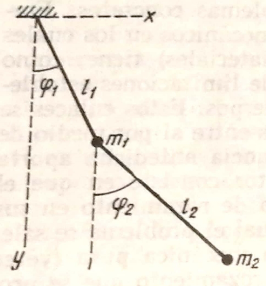
\includegraphics[width=0.3\textwidth]{img/pregunta_1.png}
  \caption{Péndulo Doble}
  \label{fig:pregunta_1}
\end{figure}

En este caso, tenemos $3 \cdot N = 3\cdot 2 = 6$ coordenadas cartesianas. Sin embargo, tenemos las siguientes ligaduras:
\begin{enumerate}
  \item $z = 0$
  \item  $l_1 = cte$
  \item $l_2 = cte$
\end{enumerate}

Por lo cual tenemos $3N - n = 3 \cdot 2 - 4 = 2$. Por lo tanto tenemos dos grados de libertad. Con esto entonces definamos las coordenadas generalizadas de la manera en la que nos propone la imagen \ref{fig:pregunta_1}. Con lo cual nos queda:
\begin{align*}
  x_1 &= l_1\cdot \sin\left(\varphi_1\right)  \implies \dot{x_1} = l_1 \dot{\varphi_1} \cos\left( \varphi_1 \right) \\
  y_1 &= -l_1\cdot \cos\left(\varphi_1\right) \implies \dot{y_1} = l_1\dot{\varphi_1}\sin\left( \varphi_1 \right) 
.\end{align*}

Dado que este primer caso es esencialmente un triangulo en donde estamos calculando los dos catetos (Note que el valor de $y$ es negativo)

Ahora bien, de manera similar, para la masa 2 esto seria como calcular estos mismos catetos. Sin embargo, debe iniciar desde los valores de $m_1$
\begin{align*}
  x_2 &= l_1\cdot \sin\left(\varphi_1\right) + l_2 \cdot \sin\left( \varphi_2 \right) \implies \dot{x_2} = l_1\dot{\varphi_1}\cos\left( \varphi_1 \right) + l_2 \dot{\varphi_2}\cos\left( \varphi_2 \right)  \\
  y_2 &= -l_1\cdot \cos\left(\varphi_1\right) - l_2 \cdot \cos\left( \varphi_2 \right) \implies \dot{y_2} = l_1\dot{\varphi_1}\sin\left( \varphi_1 \right) + l_2 \dot{\varphi_2}\sin\left( \varphi_2 \right)  \\
.\end{align*}

Con esto entonces, podemos calcular la energía cinética que es:
\begin{align*}
  T_1 &= \frac{1}{2}m_1v_1^2 \\
      &= \frac{1}{2}m_1\left( \dot{x}_1^2 + \dot{y}_1^2 \right)  \\
      &= \frac{1}{2}m_1\left( l_1^2\dot{\varphi_1}^2\cos^2\left( \varphi_1 \right) + l_1^2\dot{\varphi_1}^2 \sin^2\left( \varphi \right)  \right)  \\
      &= \frac{1}{2}m_1\left( l_1^2\dot{\varphi_1}^2 \right)\left( \cos^2\left( \varphi_1 \right) + \sin^2\left( \varphi_1 \right)  \right)   \\
      &= \frac{1}{2}m_1\left( l_1^2\dot{\varphi_1}^2 \right)
.\end{align*}

Y
\begin{align*}
  T_2 &= \frac{1}{2}m_2v_2^2 \\
      &= \frac{1}{2}m_2\left( \dot{x}_2^2 + \dot{y}_2^2 \right)  \\
      &= \frac{1}{2}m_2 \left( \left( l_1\dot{\varphi_1}\cos\left( \varphi_1 \right) + l_2 \dot{\varphi_2}\cos\left( \varphi_2 \right) \right)^2 + \left( l_1\dot{\varphi_1}\sin\left( \varphi_1 \right) + l_2 \dot{\varphi_2}\sin\left( \varphi_2 \right) \right)^2  \right)  \\
  \left( l_1\dot{\varphi_1}\cos\left( \varphi_1 \right) + l_2\dot{\varphi_2}\cos\left( \varphi_2 \right)  \right)^2 &= l_1^2\dot{\varphi_1}^2\cos^2\left( \varphi_1 \right) + 2l_1l_2\dot{\varphi_1}\dot{\varphi_2}\cos\left( \varphi_1 \right)\cos\left( \varphi_2 \right) + l_2^2\dot{\varphi_2}^2\cos^2\left( \varphi_2 \right)  \\
  \left( l_1\dot{\varphi_1}\sin\left( \varphi_1 \right) + l_2\dot{\varphi_2}\sin\left( \varphi_2 \right)  \right)^2 &= l_1^2\dot{\varphi_1}^2\sin^2\left( \varphi_1 \right) + 2l_1l_2\dot{\varphi_1}\dot{\varphi_2}\sin\left( \varphi_1 \right)\sin\left( \varphi_2 \right) + l_2^2\dot{\varphi_2}^2\sin^2\left( \varphi_2 \right)  \\
  l_1^2\dot{\varphi_1}^2\sin^2\left( \varphi_1 \right) + l_1^2\dot{\varphi_1}^2\cos^2\left( \varphi_1 \right)^2 &= l_1^2\dot{\varphi_1}^2\left( \sin^2\left( \varphi_1 \right) + \cos^2\left( \varphi_1 \right)  \right)  \\
														&\implies l_1^2 \dot{\varphi_1}^2 \\
  l_2^2\dot{\varphi_2}^2\sin^2\left( \varphi_2 \right) + l_2^2\dot{\varphi_2}^2\cos^2\left( \varphi_2 \right)^2 &= l_2^2\dot{\varphi_2}^2\left( \sin^2\left( \varphi_2 \right) + \cos^2\left( \varphi_2 \right)  \right)  \\
														&\implies l_2^2\dot{\varphi_2}^2 \\
  2l_1l_2\dot{\varphi_1}\dot{\varphi_2}\cos\left( \varphi_1 \right)\cos\left( \varphi_2 \right) &+ 2l_1l_2\dot{\varphi_1}\dot{\varphi_2}\sin\left( \varphi_1 \right)\sin\left( \varphi_2 \right) = 2l_1l_2\dot{\varphi_1}\dot{\varphi_2}\left( \cos\left( \varphi_1 \right)\cos\left( \varphi_2 \right) + \sin\left( \varphi_1 \right)\sin\left( \varphi_2 \right)  \right) \\
												&\implies 2l_1l_2\dot{\varphi_1}\dot{\varphi_2}\cos\left( \varphi_1 - \varphi_2 \right)  \\
												&= \frac{1}{2}m_2\left( l_1^2\dot{\varphi_1}^2 + l_2^2\dot{\varphi_2}^2  + 2l_1l_2\dot{\varphi_1}\dot{\varphi_2}\cos\left( \varphi_1 - \varphi_2 \right)\right) 
.\end{align*}

Ahora bien, para el caso de la energía potencial tenemos
\begin{align*}
  V_1 &= m_1gy_1 \\
  &= -m_1gl_1\cos\left( \varphi_1 \right)  \\
  V_2 &= m_2g y_2 \\
  &= -m_2g\left( l_1\cos\left( \varphi_{1} \right) + l_2\cos\left( \varphi_2 \right)  \right) 
.\end{align*}

Ahora bien, tenemos entonces que:
\begin{align*}
  T &= T_1 + T_2 \\
    &= \frac{1}{2}m_1\left( l_1^2\dot{\varphi}_1^2 \right) + \frac{1}{2}m_2\left( l_1^2\dot{\varphi_1}^2 + l_2^2\dot{\varphi_2}^2  + 2l_1l_2\dot{\varphi_1}\dot{\varphi_2}\cos\left( \varphi_1 - \varphi_2 \right)\right) \\
    &= \frac{1}{2}l_1^2\dot{\phi_1}^2\left( m_1 + m_2 \right) + \frac{1}{2}m_2l_2^2\dot{\phi_2}^2 + m_2l_1l_2\dot{\varphi_1}\dot{\varphi_2}\cos\left( \varphi_1 - \varphi_2 \right) 
.\end{align*}

Y
\begin{align*}
  V &= V_1 + V_2 \\
  &= -m_1gl_1\cos\left( \varphi_1 \right) -m_2gl_1\cos\left( \varphi_1 \right) - m_2gl_2\cos\left( \varphi_2 \right)  \\
  &= - gl_1\cos\left( \varphi_1 \right) \left( m_1 + m_2 \right) - m_2 gl_2\cos\left( \varphi_2 \right)
.\end{align*}

Por lo tanto dado que $L = T - V$ nos queda:
\begin{align*}
  L &= T - V \\
  L &=  \frac{1}{2}l_1^2\dot{\phi_1}^2\left( m_1 + m_2 \right) + \frac{1}{2}m_2l_2^2\dot{\phi_2}^2 + m_2l_1l_2\dot{\varphi_1}\dot{\varphi_2}\cos\left( \varphi_1 - \varphi_2 \right) -\left( - gl_1\cos\left( \varphi_1 \right) \left( m_1 + m_2 \right) - m_2 gl_2\cos\left( \varphi_2 \right) \right)  \\
   &=  \frac{1}{2}l_1^2\dot{\phi_1}^2\left( m_1 + m_2 \right) + \frac{1}{2}m_2l_2^2\dot{\phi_2}^2 + m_2l_1l_2\dot{\varphi_1}\dot{\varphi_2}\cos\left( \varphi_1 - \varphi_2 \right) +  gl_1\cos\left( \varphi_1 \right) \left( m_1 + m_2 \right) + m_2 gl_2\cos\left( \varphi_2 \right)
.\end{align*}

\chapter{}

En este caso vamos a partir de que un cilindro rueda sobre otro. Para este caso tenemos dos cilindros, uno de radio $a$  y uno de radio $\alpha a$. Las medidas se pueden observar en la figura \ref{fig:img-pregunta_3_1-png}. 

\begin{figure}[H]
  \centering
  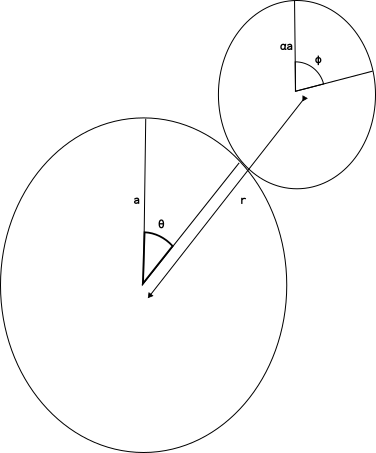
\includegraphics[width=0.4\textwidth]{img/pregunta_3_1.png}
  \caption{Dimensiones y descripción del problema}
  \label{fig:img-pregunta_3_1-png}
\end{figure}

Con esto entonces nos hace falta ver las fuerzas que las puede encontrar en la figura \ref{fig:img-pregunta_3_2-png}

\begin{figure}[H]
  \centering
  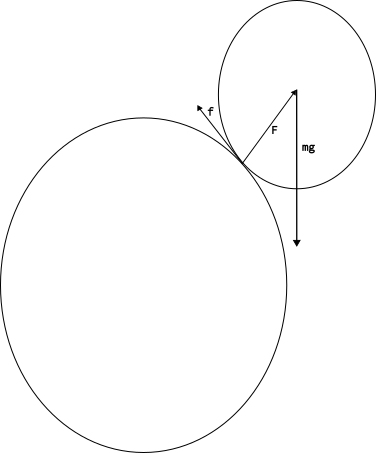
\includegraphics[width=0.4\textwidth]{img/pregunta_3_2.png}
  \caption{Fuerzas en el sistema}
  \label{fig:img-pregunta_3_2-png}
\end{figure}

En este caso, dado que el cilindro $\alpha a$ ira teniendo cada vez una menor fuerza $Z$ (dado que el angulo en el que se encuentra con respecto a su eje disminuye) entonces sabemos que eventualmente este cilindro se despegara del fijo $a$. Ademas, sabemos que estos dos perderán contacto en cuanto la fuerza normal  $F$ ya no tenga ingerencia. Es decir, cuando \[
F = 0
.\] Ademas, sabemos por el como funciona la fricción que \[
f \le \mu F
.\] donde $\mu$ es el coeficiente de fricción. Lo que implica que este movimiento eventualmente empezara a deslizar sobre la superficie. Por lo tanto, podemos dividir este análisis en 3 momentos definidos por los ángulos $\theta_1$, $\theta_2$ y $\theta_3$. Para iniciar, desde $0$ hasta $\theta_1$ el cilindro rueda sin deslizar, lo que se describe en que la fricción seria \[
f = \mu F
.\] Ahora, entre $\theta_1$ y $\theta_2$ el cilindro se deslizaría pues la fricción es muy pequeña y en $\theta_2$ el cilindro dejaría de estar en contacto con el otro y por lo tanto se sostendría $F = 0$ y de ahí en adelante caería libremente.

Ahora bien iniciemos caso a caso
\section{}

Para empezar para un movimiento que no desliza entonces sabemos que:
\begin{align*}
  a\theta &= \alpha a \left( \varphi - \theta \right) \\
  \theta &= \alpha \left( \varphi - \theta \right) \\
  \theta &= \alpha \varphi - \alpha \theta \\
  \theta + \alpha \theta &= \alpha\varphi \\
  \left( 1 + \alpha \right) \theta &= \alpha \varphi
.\end{align*}

Ahora bien, podemos definir una función desarrollando:
\begin{align*}
  \left( 1 + \alpha \right) \theta &= \alpha \varphi \\
  \theta &= \frac{\alpha \varphi}{\left( 1 + \alpha \right) } \\
  \gamma &= \theta - \frac{\alpha \varphi}{\left( 1 + \alpha \right) }
.\end{align*}

Donde, como se puede notar cuando esto no desliza $\gamma = 0$. Ahora bien, por otro lado, tenemos que al estar estos dos cilindros en contacto la distancia entre los centros queda: \[
r = a + \alpha a = \left( 1 + \alpha \right) a
.\] Ahora bien,
\begin{align*}
  T_1 &= \frac{1}{2}m \\
.\end{align*}

\end{document}
